%v4.4
\subsection{Hadron Calorimeter (HCal)}
%
\label{sec:expsetup_hcal}

The Hadron Calorimeter (HCal) has been designed specifically to measure the recoil nucleon for the SBS experiments. Specifically for this experiment (and for $G_M^n$), HCal combined with the SBS (48D48) magnet provides identification of the recoil nucleon, as well as additional kinematic constraint and possibly timing information on the measured interaction.
Nucleon identification is illustrated on Fig.~\ref{fig:hcal_nuclimprint}. This figure shows the compared proton and neutron position distribution in HCal at the same electron kinematics. The proton distribution is being shifted upwards by about $1~\mathrm{m}$ compared to the neutron.
%
\begin{figure}[!h]
  \begin{center}
    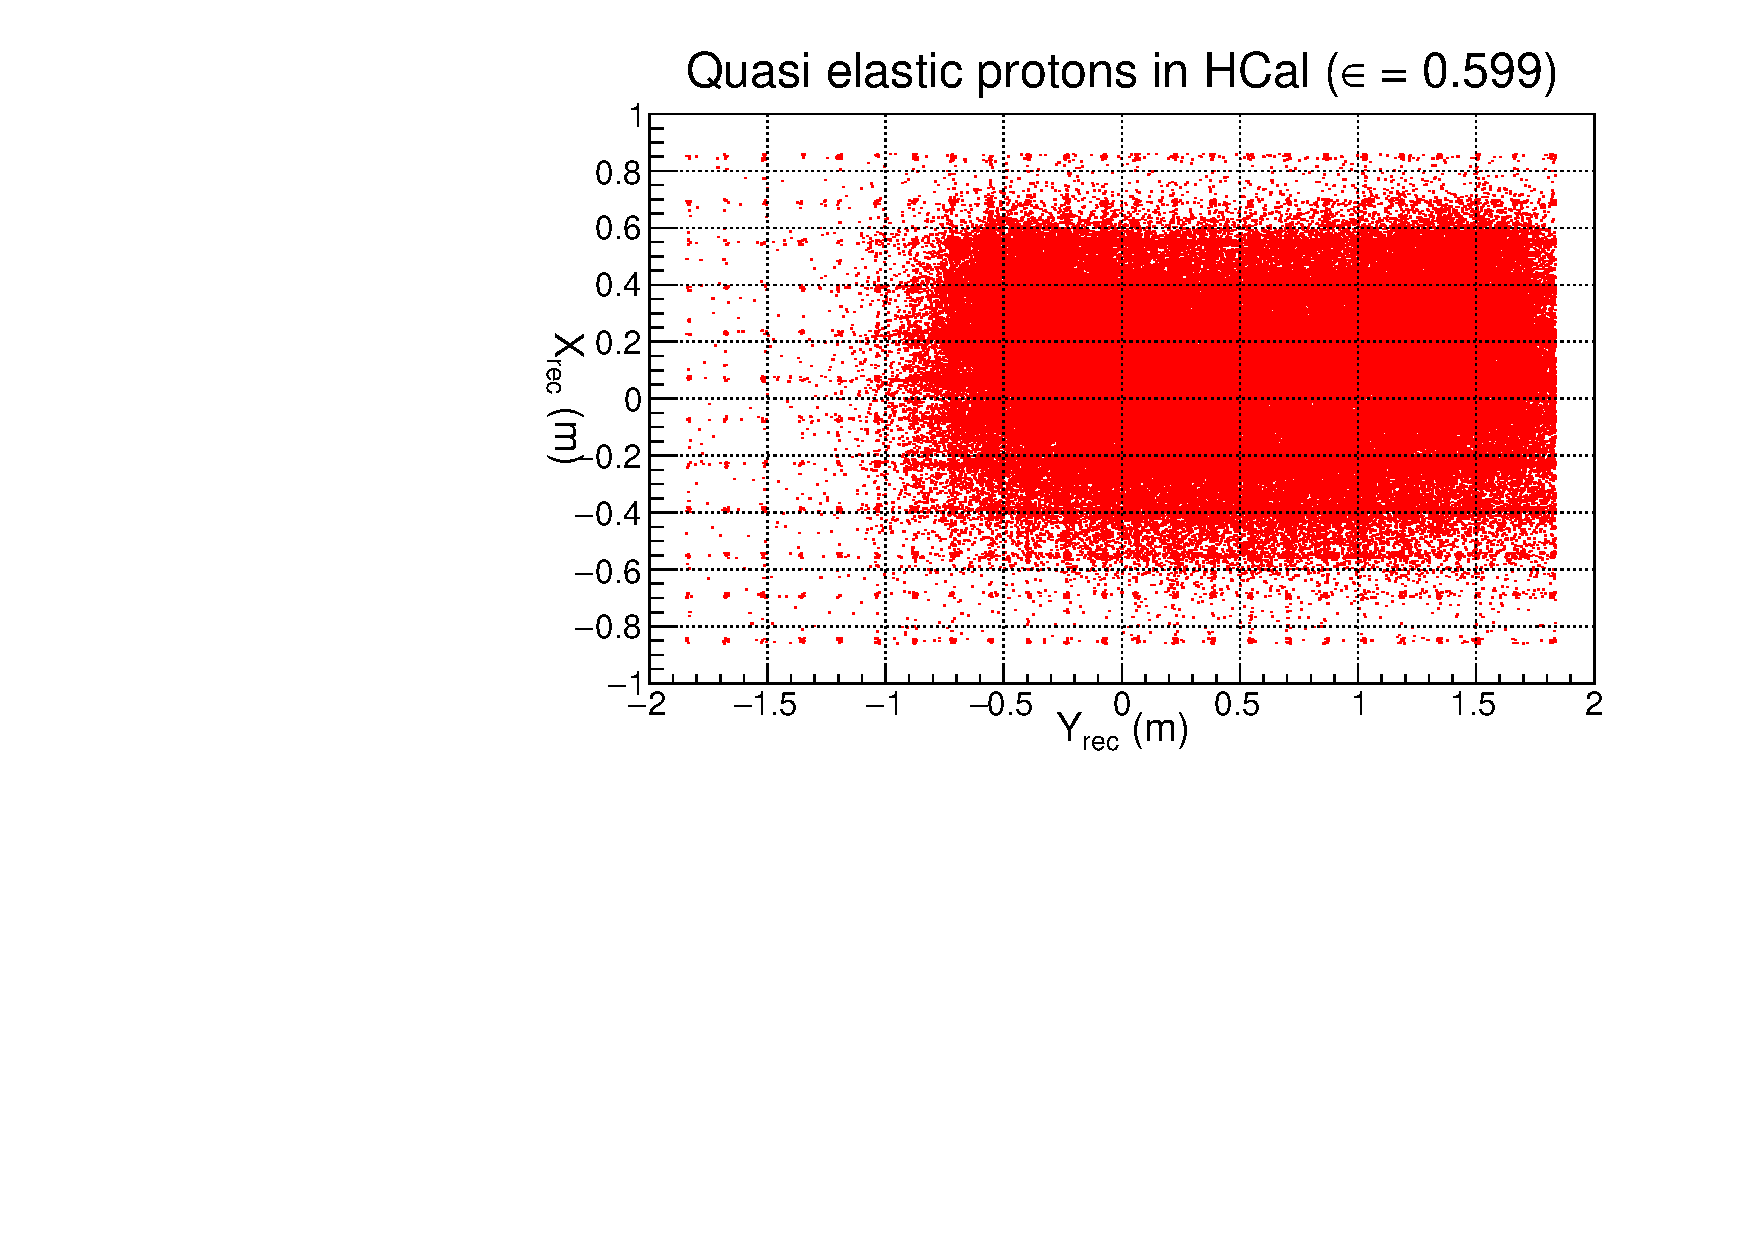
\includegraphics[angle=90,width=4cm]{Plots/HCal_p.pdf}
    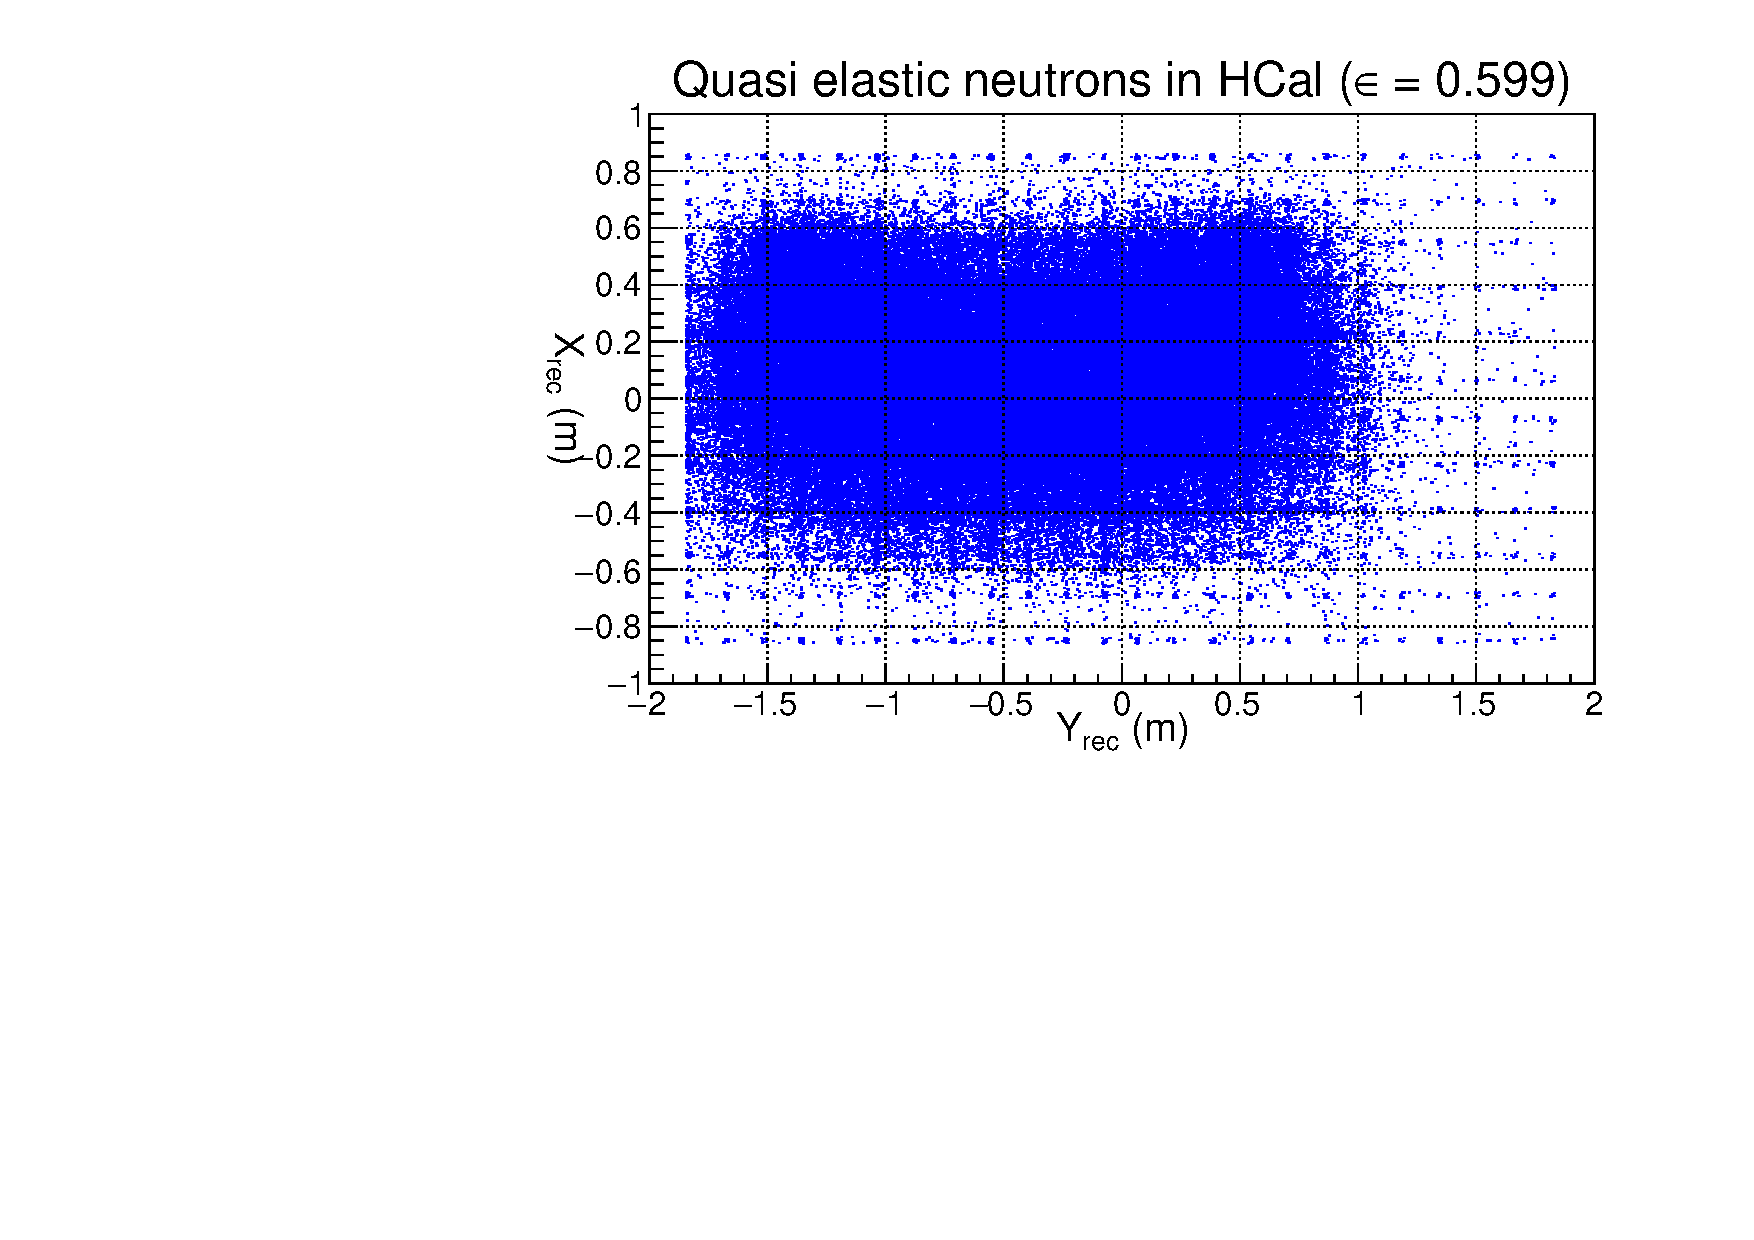
\includegraphics[angle=90,width=4cm]{Plots/HCal_n.pdf}
    \caption{Reconstructed HCal cluster from quasi-elastic events generated by G4SBS. The left distribution in red is for the proton, the right distribution in blue is for the neutron.}
    \label{fig:hcal_nuclimprint}
  \end{center}
\end{figure}
%

%\subsubsection{Structure of the HCal}

The HCal (which CAD model is shown on Fig.~6)%\ref{fig:hcal_cad})
is composed of 288 modules arranged in an array of $12\, \times \, 24$
%
\begin{figure}[!h]
  \begin{center}
    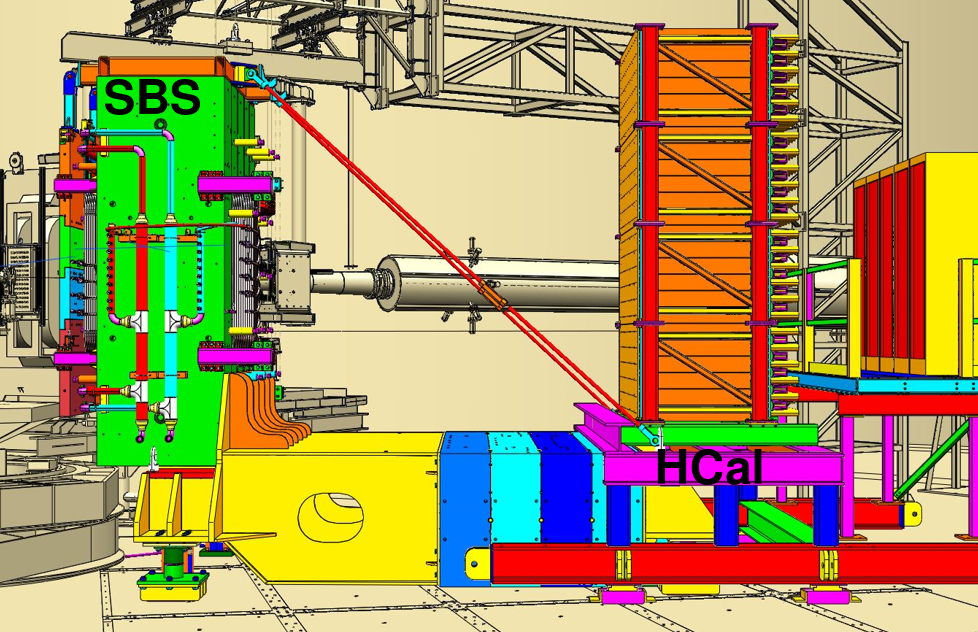
\includegraphics[width=10cm]{Plots/Wines_SBS_CAD_Fall2018.png}
    \caption{CAD representation of HCal (right) with the SBS magnet (left)}
    \label{fig:hcal_cad}
  \end{center}
\end{figure}
%
In front of the full assembly is located a $3/4~\mathrm{in}$ steel plate which purpose is double:
%
\begin{itemize}
\item{initiate the hadronic shower to optimize the calorimeter response;}
\item{shield the modules from a fraction of the low energy secondaries;}
\end{itemize}
%
Each of these modules measures $6\,\times~6\,\mathrm{in}^2$ section, for $3~\mathrm{ft}$ length. They are composed of alternating tiles of scintillators and iron around a central light guide which collects the light generated in the scintillators by the hadronic shower, and guides it to the PMT at the end of the block.
Cosmics tests have determined that the average light yield for the HCal modules is around 5 photoelectrons per MeV deposited in the scintillator tiles.

The PMTs are readout with FADC250 which sample the PMT signal every 4 ns and allow to reconstruct the PMT pulse shape, hence its timing.
They are also readout by TDCs which provide additional timing information.
Thanks to this, the timing resolution can be better than $1~\mathrm{ns}$, which cosmics tests (in progress) seem to confirm.

The energy resolution is intrinsically broad (see Fig.~\ref{fig:HCalRates} in Section~\ref{sec:simu}), due mostly to the small fraction of energy from the hadronic shower actually measured by the scintillator tiles ($\leq 0.1$ - refer yet again to Fig.~\ref{fig:HCalRates}).

%Note that the photoelectron statistics in the PMTs should not be a huge contributor to the resolution width. 
%\subsubsection{Parameters of the HCal}
\iffalse
The HCal angle and distance to the target will move from a kinematic to the other. At 8.5 m which is the largest distance for this experiment, the solid angle from the target is about 90 msr.
The matching between the electron in BigBite and the nucleon in HCal is about 90\% for the low $\epsilon$ kinematic.
For the high $\epsilon$ kinematic, HCal has to be brought closer to the target because the nucleon imprint is larger (Fig.~\ref{fig:hcal_nuclimprint2}).
%\iffalse
%
\begin{figure}[!h]
  \begin{center}
    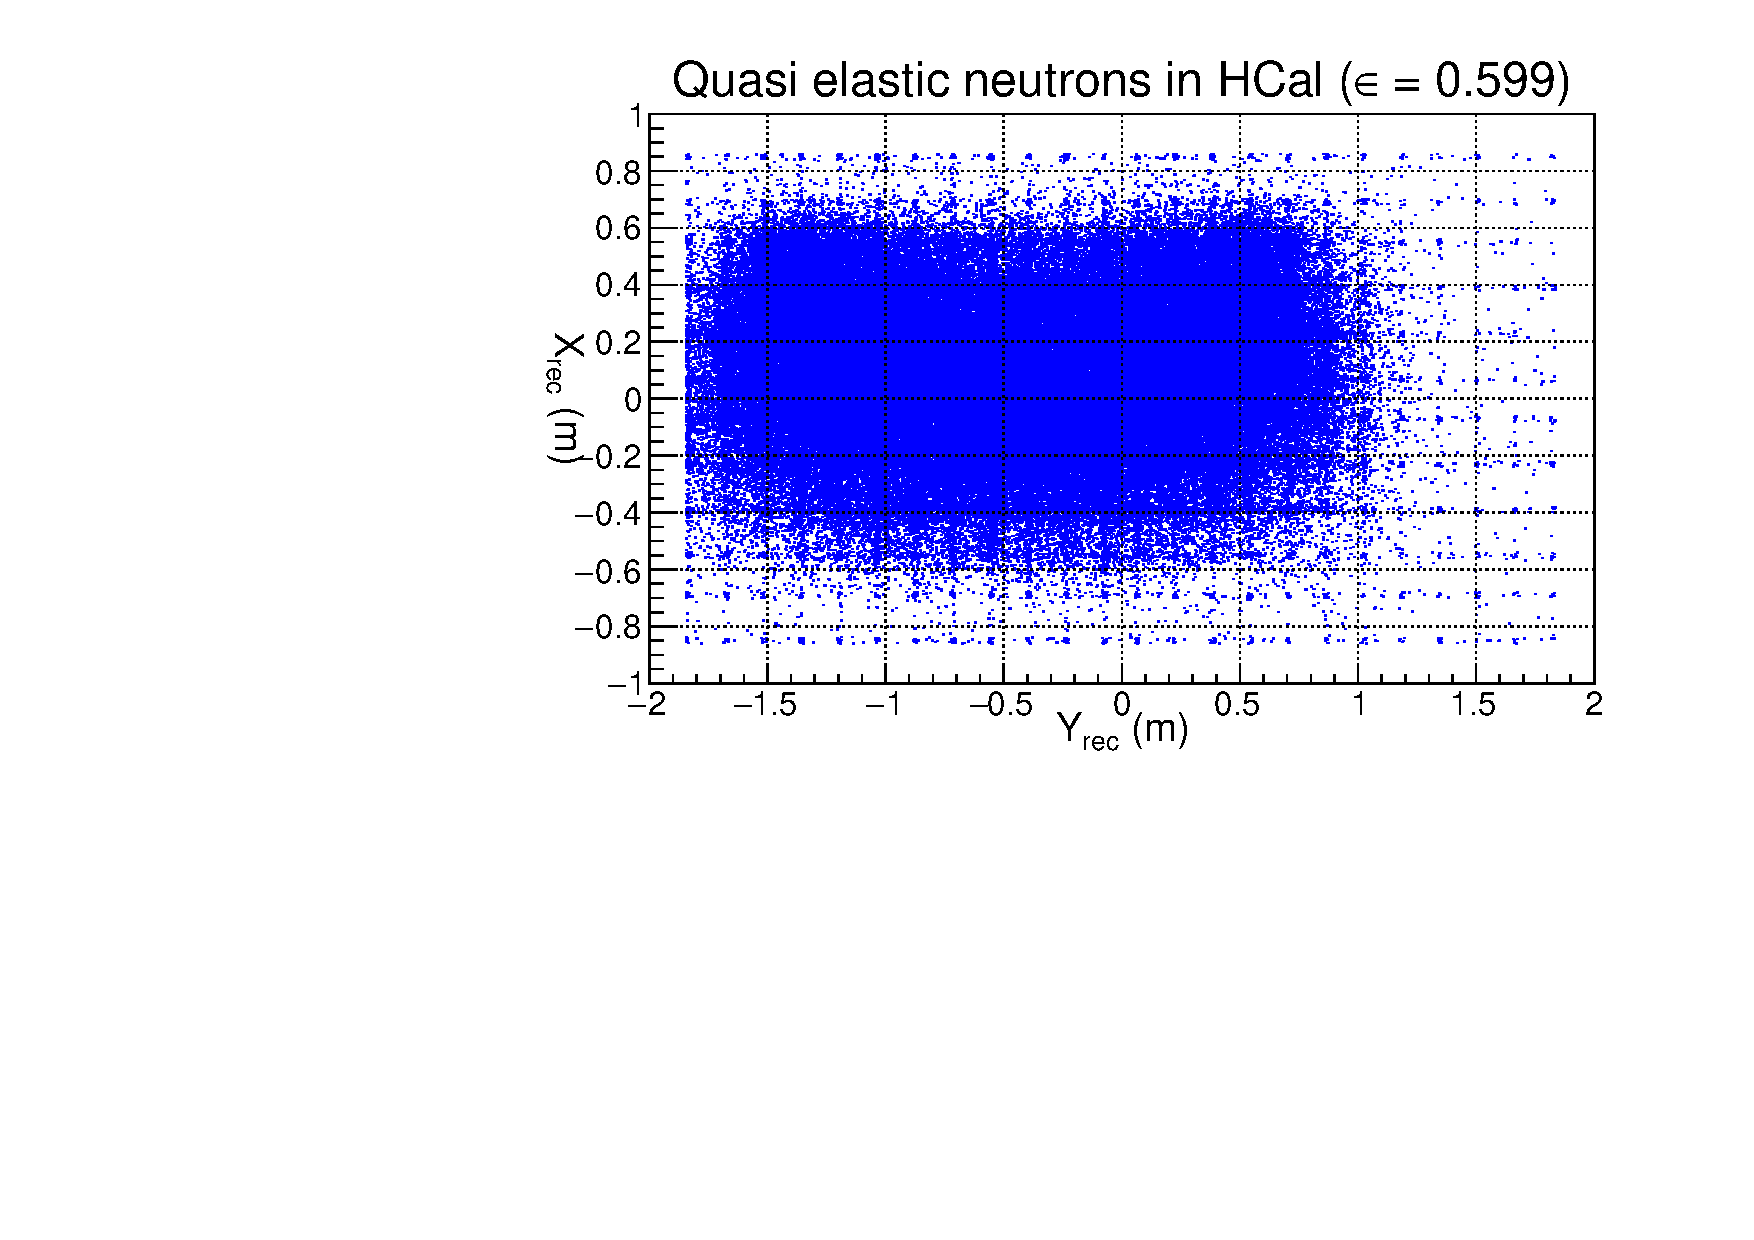
\includegraphics[angle=90,width=4cm]{Plots/HCal_n.pdf}
    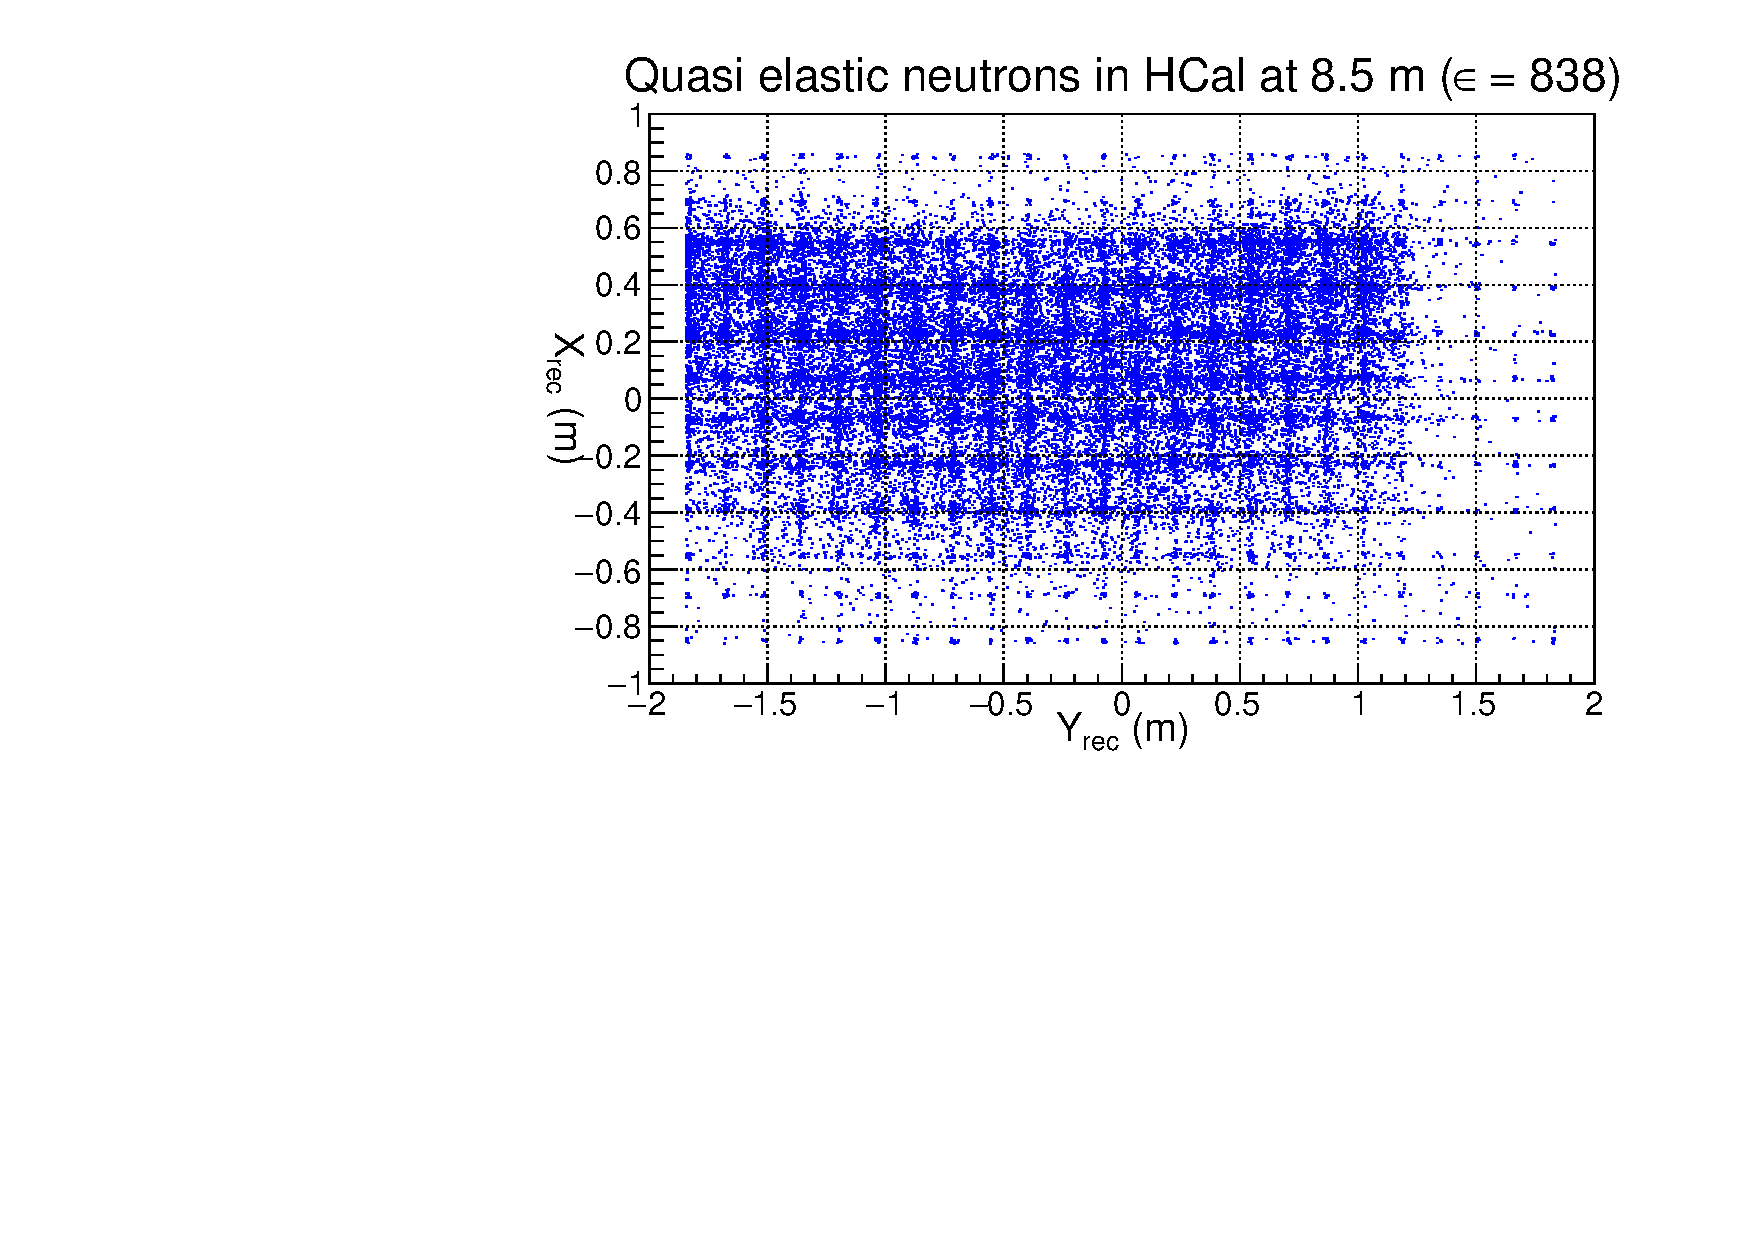
\includegraphics[angle=90,width=4cm]{Plots/HCal_n_he.pdf}
    \caption{Reconstructed HCal cluster from quasi-elastic events generated by G4SBS. The left distribution is for the neutron at the low $\epsilon$ kinematic, the right distribution is for the neutron at the high $\epsilon$ kinematic, and the same distance from the target.}
    \label{fig:hcal_nuclimprint2}
  \end{center}
\end{figure}
%
\fi

